
\newpage
\subsection{Схема базы данных}
\textbf{Номера уровней последовательности заполнения базы данных.}
\begin{enumerate}
    \item <<Порода>>, <<Фаза лактации>>, <<Сезонность>>, <<Суточность>>, <<Зоотехник>>, <<Вид корма>>.
    \item <<Корова>>, <<Рацион>>, <<Корм>>. 
    \item <<Питание>>, <<Лактация>>.
    \item <<План кормления>>.
\end{enumerate}

На рисунке \ref{fig:уровни} представлена схема уровней заполнения базы данных.
\begin{figure}[H]
    \centering
    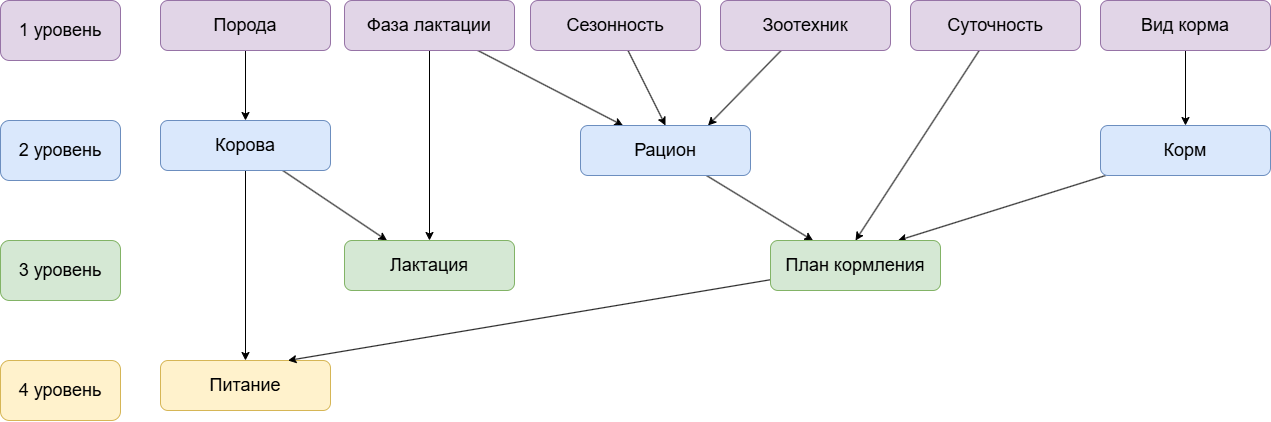
\includegraphics[width=1\linewidth]{схема уровней_бд.png}
    \caption{Схема уровней заполнения базы данных}
    \label{fig:уровни}
\end{figure}
На рисунке \ref{fig:схема_бд} представлена схема базы данных на русском языке. 
На рисунке \ref{fig:схема_бд_англ} представлена схема базы данных на английском языке. 
\clearpage
\newgeometry{margin=1cm}
\begin{landscape}
    \begin{figure}[p]
        \centering
        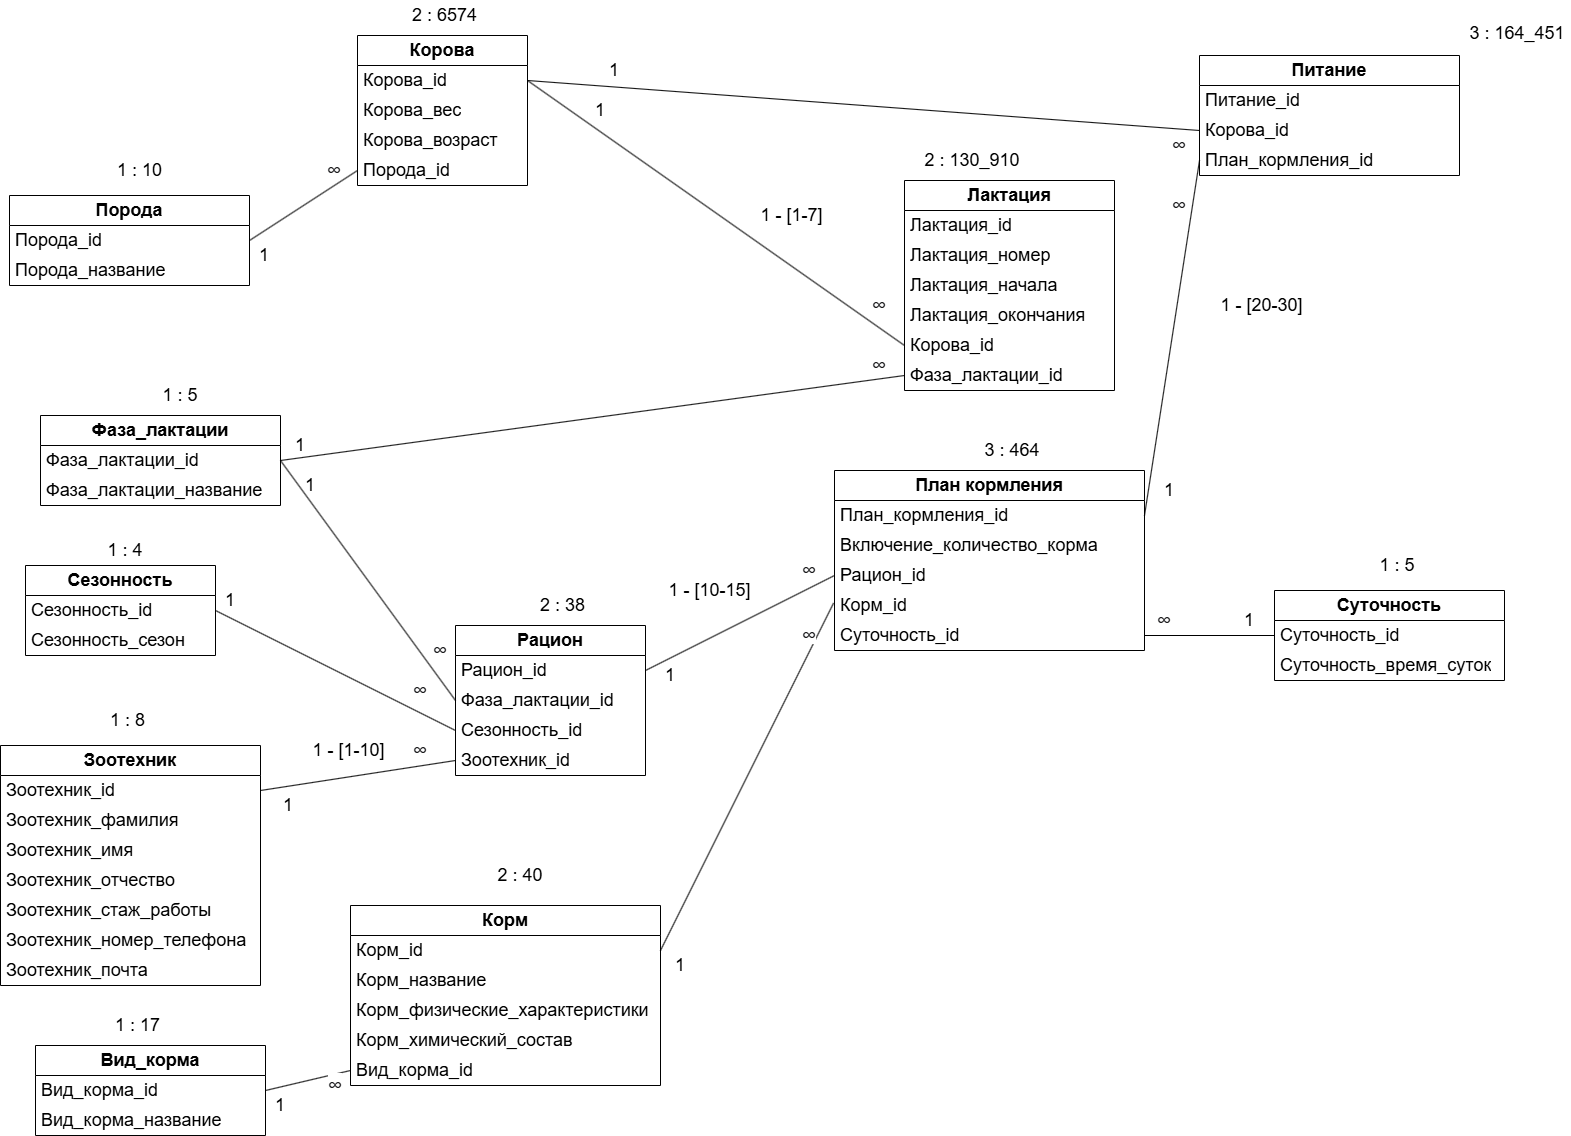
\includegraphics[width=\textwidth, height=\textheight, keepaspectratio]{схема_бд_рус.png}
        \caption{Схема базы данных на русском языке}
        \label{fig:схема_бд}
    \end{figure}
\end{landscape}
\restoregeometry
\clearpage

\clearpage
\newgeometry{margin=1cm}
\begin{landscape}
    \begin{figure}[p]
        \centering
        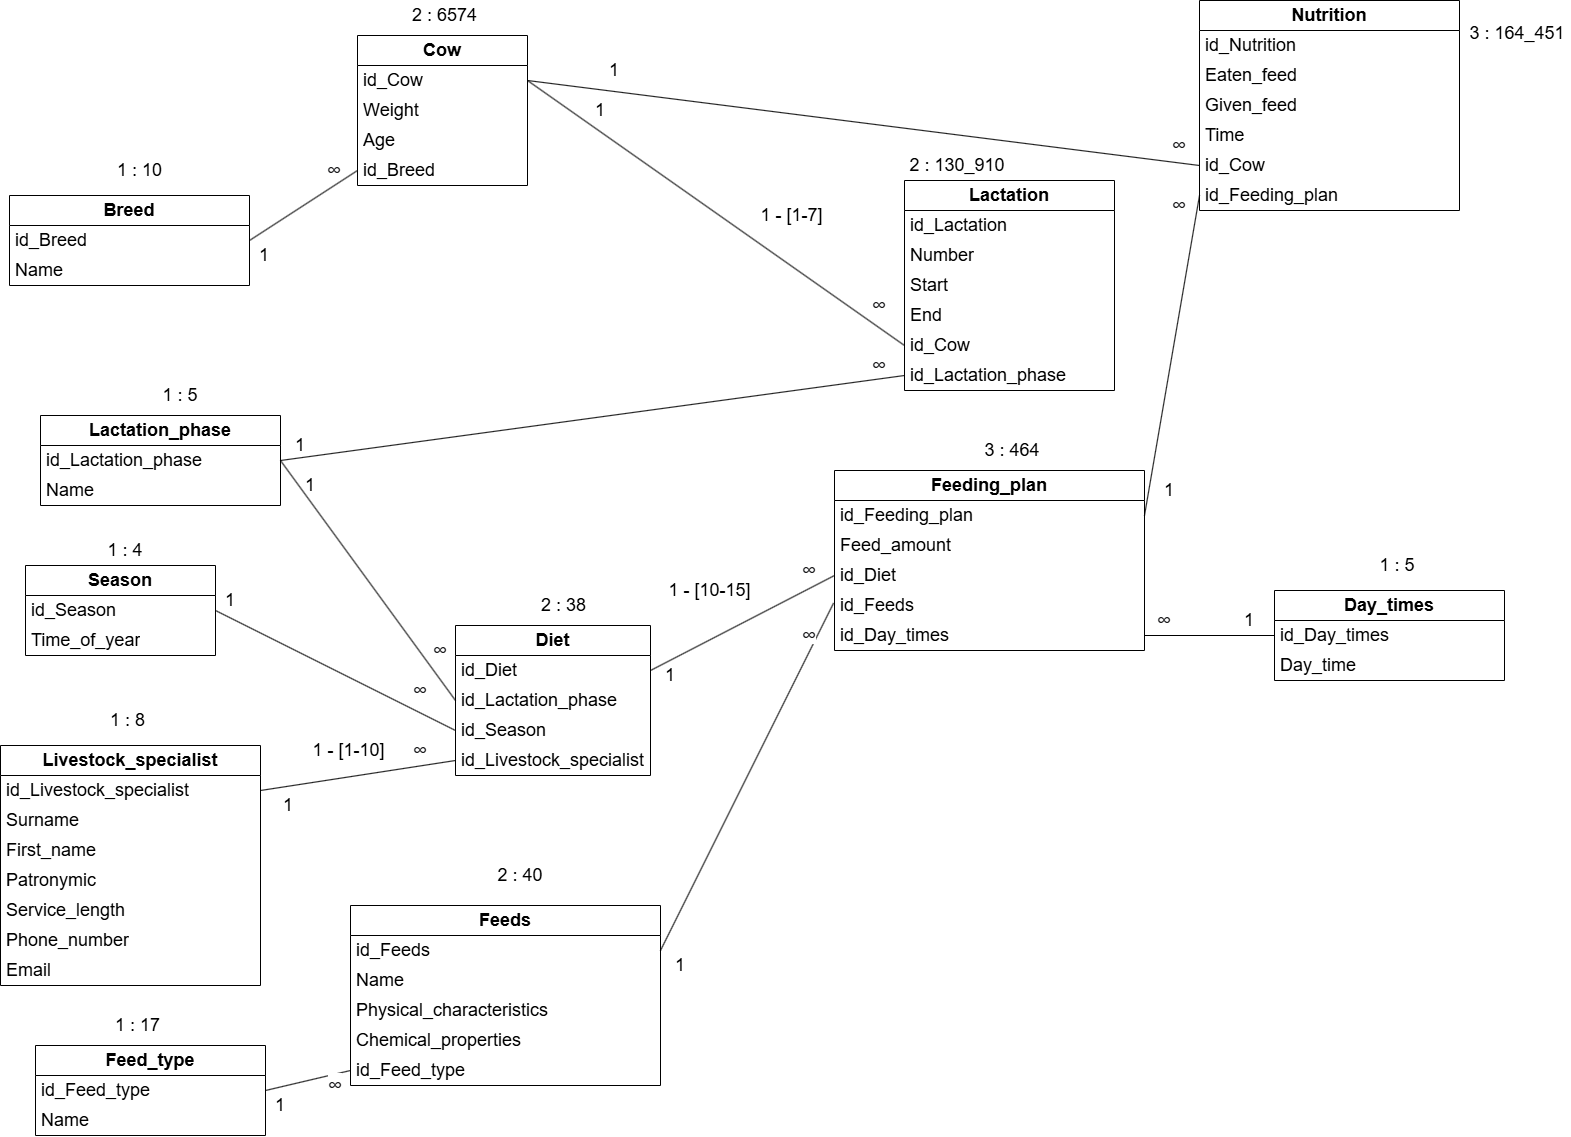
\includegraphics[width=\textwidth, height=\textheight, keepaspectratio]{схема_бд_англ.png}
        \caption{Схема базы данных на английском языке}
        \label{fig:схема_бд_англ}
    \end{figure}
\end{landscape}
\restoregeometry
\clearpage